The XADD~\cite{sanner_uai11} data structure is an extension of ADD, that allows greater expressivity, representing symbolic piecewise polynomials. More specifically, the functions that are represented in a XADD are of the form $f : \{ 0, 1\}^n\times \mathbb{R}^m \rightarrow \mathbb{E}(\mathbb{R}^m)$, where $\mathbb{E}(\mathbb{R}^m)$ denotes the set of expressions containing real-valued constants and the continuous variables related by operations of addition or multiplication.

Here is the formal definition of XADDs as a BNF grammar:

$<$Node$>$ $=$ Internal $|$ Terminal.\\
$<$Terminal$>$ $=$ TermExpr.\\
$<$Expr$>$ $=$ Term $|$ Term "+" Expr.\\
$<$Term$>$ $=$ $c \prod_{i=1}^m {x_i^{\alpha_i }}$.\\
$<$Internal$>$ $=$ Decision "?" highNode  ":" lowNode.\\
$<$Decision$>$ $=$ $b_k$ $|$ Ineq.\\
$<$Ineq$>$ $=$ IneqExpr "$>$" 0.\\

Here, $b_k$ is a boolean variable, and $x_i$ are the continuous variables in this XADD. $c$ is a real number, $\alpha_i$ are positive integers, highNode and lowNode are elements of the Node grammar and TermExpr and IneqExpr are elements of the Expr grammar.
For the case of linear XADDs, the generation rule for continuous expressions is simplified: $<$Expr$>$ $=$ $\vec{c}\cdot\vec{x_0}$ $:=$ $\sum_{i=0}^m {c_i x_i}$.\\
where $c_i$ are real values and $x_0$ is simply 1, and $\vec{x_0} = (x_0 = 1 ,x_1,..., x_m)$, a convenient notation that allows us to add in a constant to linear functions. We observe that in the linear case, the expression set $\mathbb{E}_{lin}(\mathbb{R}^m)$ is equivalent to $\mathbb{R}^{m+1}$, as each linear expression corresponds uniquely to a coefficient vector $\vec{c} = (c_0, ..., c_m)$.

In order to identify equivalent inequalities, we require that the inequality expressions are normalized, that is, the terms are ordered according to a continuous variable ordering, and the leading term must have either 1 or -1 as it coefficient.
Additional restrictions are that the "Decision" in an internal node cannot appear in its descendent nodes and must follow a decision ordering. It is important to note that the variable ordering in ADDs is extended to a decision ordering in XADDs, and though the number of different decisions is possibly infinite (as there are infinite different inequalities) the number of decisions present in a finite set of XADDs is finite and can be ordered by enumeration.

The evaluation $V(\cdot, \rho)$ of a XADD to a real value under a variable assignment $\rho = (\rho^b,\rho^x)$ is defined recursively as follows:

{\footnotesize
$V(\text{Term},\rho) = c \cdot \prod_{i=1}^m { (\rho^x_i)^{\alpha_i}}$\\
$V(\text{Expr},\rho)) = \sum_k V(\text{Term}_k, \rho)$\\
$V(\text{Internal},\rho) = \begin{cases} 
if \text{ }V(\text{Decision},\rho) = true:  V(\text{highNode},\rho)\\
if \text{ }V(\text{Decision},\rho) = false:  V(\text{lowNode},\rho)\\
\end{cases} $\\
$V(b_k, \rho) =$ $true$ $if$ $\{ b_k = 1\} \in \rho^b$ : $false$ $otherwise$\\
$V(\text{Ineq},\rho) =$ $true$ $if$ $V(\text{IneqExpr},\rho) > 0 $ : $false$ $otherwise$\\
}

In the Figure \ref{fig:xaddex} we give an example of XADD, and how it is evaluated for a variable assignment.

\begin{figure}[h!t]
\center
\fbox{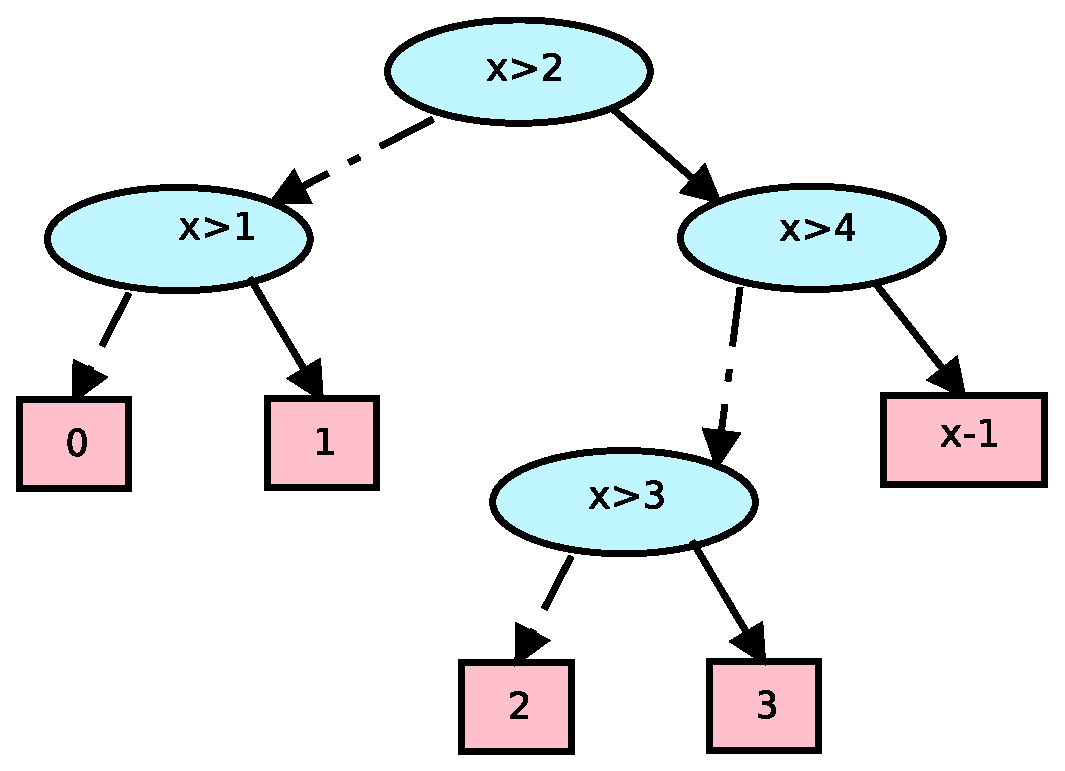
\includegraphics[scale=0.4]{Figures/xadds/samplexadd.eps} }
\caption{ Example of XADD.}
\label{fig:xaddex} 
\end{figure}


%%%%%%%%%%%%%%%%%%%%%%%%%%%%%%%%%%%%%%%%%%%%%%%%%%%%%%%%%%%%%%%%%%%
%%%%%%%%%%%%%%%%%%%%%%%%%%%%%%%%%%%%%%%%%%%%%%%%%%%%%%%%%%%%%%%%%%%




Binary operations as addition and multiplication can be performed in
XADD analogously to the ADD version, as the expressions themselves
support this operations. The division operation, however, is not
closed in polynomial expressions, and thus is not supported in
polynomial XADDs. The boolean variable marginalization simply involves
an addition so is also supported. Still, unary maximization or
minimization involves obtaining extremum from arbitrary polynomials,
and thus is only supported in exact form for linear XADDs. An
operation that requires detailed description is the binary
maximization. It is closed form both in linear and polynomial XADDs,
but introduce new decisions. We define \emph{symbolic binary
maximization} in the case representation as follows, and illustrate it
as an XADD operation in figure~\ref{fig:xaddmax}:

\begin{figure}[h!t]
\center
\fbox{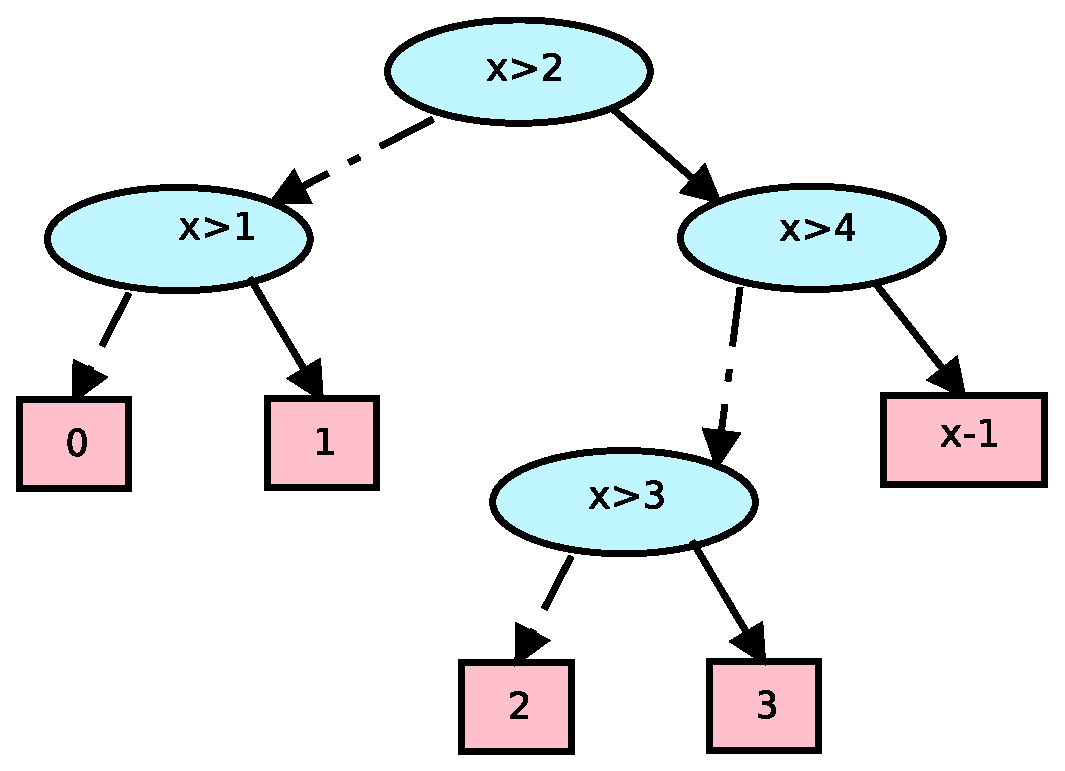
\includegraphics[scale=0.4]{Figures/xadds/samplexadd.eps} }
\caption{ Example of XADD max Operation.}
\label{fig:xaddmax} 
\end{figure}


\vspace{-5mm}
{\footnotesize
\begin{center}
\begin{tabular}{r c c c l}
&
\hspace{-7mm} $\casemax \Bigg(
  \begin{cases}
    \phi_1: \hspace{-2mm} & \hspace{-1mm} f_1 \\ 
    \phi_2: \hspace{-2mm} & \hspace{-1mm} f_2 \\ 
  \end{cases}$
$,$
&
\hspace{-4mm}
  $\begin{cases}
    \psi_1: \hspace{-2mm} & \hspace{-1mm} g_1 \\ 
    \psi_2: \hspace{-2mm} & \hspace{-1mm} g_2 \\ 
  \end{cases} \Bigg)$
&
\hspace{-4mm} 
$ = $
&
\hspace{-4mm}
  $\begin{cases}
  \phi_1 \wedge \psi_1 \wedge f_1 > g_1    : & \hspace{-2mm} f_1 \\ 
  \phi_1 \wedge \psi_1 \wedge f_1 \leq g_1 : & \hspace{-2mm} g_1 \\ 
  \phi_1 \wedge \psi_2 \wedge f_1 > g_2    : & \hspace{-2mm}f_1 \\ 
  \phi_1 \wedge \psi_2 \wedge f_1 \leq g_2 : & \hspace{-2mm} g_2 \\ 
  \hspace{1cm}\vdots \hspace{8mm}: & \hspace{-2mm} \vdots
  \end{cases}$
\end{tabular}
\end{center}
\vspace{-3mm}
} If all $f_i$ and $g_i$ are linear,
the $\casemax$ result is clearly still linear and representable in the case format previously described (i.e., linear inequalities in decisions).

In the rest of the paper, we will consider only linear XADDs, i.e. XADD with only linear expressions on the continuous variables, because linear XADDs permit LP solvers to be used in two ways: linear constraint feasibility checking to prune unreachable paths in the XADD and linear constrained optimization of linear functions to obtain maximum and minimum values of a XADD. Besides, our main contribution in this paper is the development of an bounded error approximation method for piecewise linear functions that is used in linear XADDs to increase efficiency.
